\section{Introdução} \label{sec:introducao}

Batalhas intergaláticas são acontecimentos constantes em um futuro distante da humanidade. Frotas de naves espaciais são enviadas para combater forças inimigas em uma guerra cruel e infindável. O planejamento de um ataque surpresa a uma frota inimiga envolve duas atividades de suma importância: o reconhececimento de naves da frota inimiga e o cálculo do tempo de vantagem (tempo mínimo até todos os tripulantes das naves atingirem seu posto de trabalho correto e se prepararem para o ataque). Deseja-se que estas duas atividades sejam realizadas da melhor forma possível, logo o trabalho de alunos de Projeto e Análise de Algoritmos da UFMG foi requisitado.


\begin{figure*}[ht]
	\centering
	\begin{subfigure}[b]{0.24\textwidth}
		\centering
		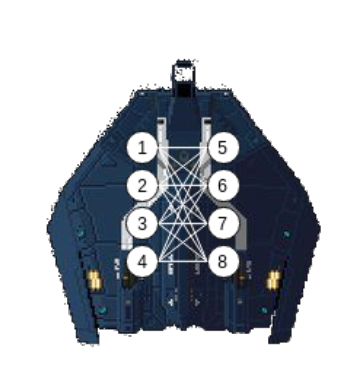
\includegraphics[width=0.9\textwidth]{imgs/bomb.png}
		\caption{Nave Bombardeira}
		\label{fig:nave_bomb}
	\end{subfigure}
	\begin{subfigure}[b]{0.24\textwidth}
		\centering
		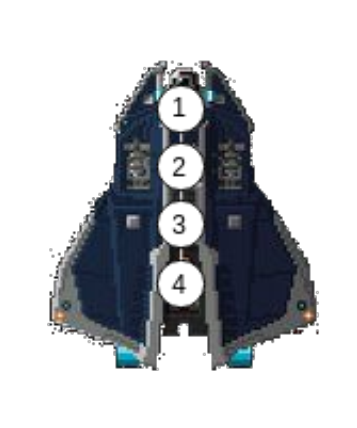
\includegraphics[width=0.9\textwidth]{imgs/rec.png}
		\caption{Nave de Reconhecimento}
		\label{fig:nave_rec}
	\end{subfigure}
	\begin{subfigure}[b]{0.24\textwidth}
		\centering
		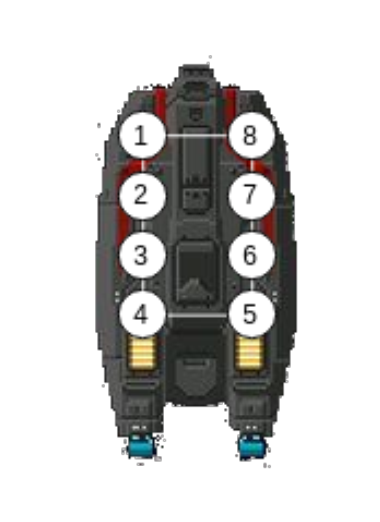
\includegraphics[width=0.9\textwidth]{imgs/trans.png}
		\caption{Nave de Transporte}
		\label{fig:nave_transp}
	\end{subfigure}
	\begin{subfigure}[b]{0.24\textwidth}
		\centering
		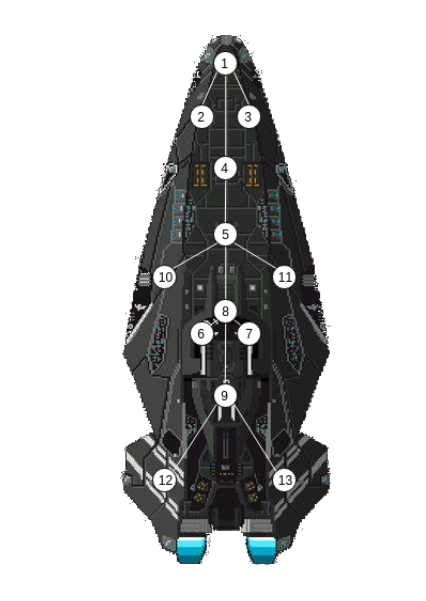
\includegraphics[width=0.9\textwidth]{imgs/frig.png}
		\caption{Nave Frigata}
		\label{fig:nave_frig}
	\end{subfigure}
	\caption{Tipos de Naves da Frota Inimiga}
	\label{fig:naves_tipos}
\end{figure*}


Sabe-se que as frotas inimigas são divididas em quatro tipos de naves, ilustrados na figura \ref{fig:naves_tipos}: \textit{Bombardeiros} (\ref{fig:nave_bomb}),  \textit{Reconhecimento} (\ref{fig:nave_rec}),  \textit{Transportadoras} (\ref{fig:nave_transp}) e \textit{Frigatas} (\ref{fig:nave_frig}). Algumas restrições são impostas a estas naves, por exemplo: em uma nave bombardeira, cada fileira de postos deve possuir no mínimo dois postos de combate; já nas naves de reconhecimento e transporte, o teleporte só é possível entre postos diretamente adjacentes.

Sabe-se também que estas naves são organizadas em postos de combates, de forma que cada tripulante pode ocupar apenas um posto por vez e, para se movimentar entre os postos, os tripulantes devem utilizar o sistema de teleporte nativo da nave. Este sistema de teleporte funciona trocando dois tripulantes por vez, entre postos de combate.

O objetivo do trabalho prático, portanto, é: dado um conjunto de pontos, representando as naves das frotas inimigas e os postos de combate presentes em cada uma delas, conexões entre estes pontos, representando as possibilidades de teleporte entre os postos, e um conjunto de pares $(p_i, p_j)$ representando teleportes a serem realizados entre dois pontos em uma mesma nave: 
\begin{itemize}
    \item Reconhecer e classificar o tipo de cada uma das naves presentes na frota inimiga
    \item Calcular o tempo de vantagem para a frota aliada (tempo mínimo para que todos os teleportes especificados pelos pares de pontos $(p_i, p_j)$ sejam realizados)
\end{itemize}


